\documentclass[tikz,margin=10pt]{standalone}
\usepackage{tikz}

\begin{document}
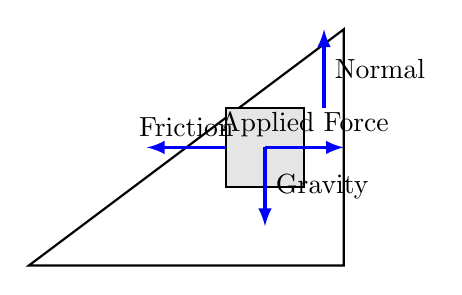
\begin{tikzpicture}[force/.style={>=latex,draw=blue,fill=blue,very thick,align=center}]

% Draw the inclined plane
\draw[thick] (0,0) -- (4,0) -- (4,3) -- cycle;

% Draw the block 
\filldraw[fill=gray!20, draw=black, thick](2.5,1) rectangle (3.5,2);

% Draw and label the forces
\draw[force, ->] (3,1.5) -- (3,0.5) node[midway,right] {Gravity};
\draw[force, ->] (2.5,1.5) -- (1.5,1.5) node[midway,above] {Friction};
\draw[force, ->] (3.75,2) -- (3.75,3) node[midway,right] {Normal};
\draw[force, ->] (3,1.5) -- (4,1.5) node[midway,above] {Applied Force};

\end{tikzpicture}
\end{document}